\section{Sving}
\label{sving}
Bilen skal deltage i en racerløb, derfor er der blevet lagt vægt på at optimere bilens kørsel. 
For at kunne optimere omgangstiden skal der benyttes flere forskellige fysiske ligninger. Disse bruges til at finde bremsepunkterne og hastighedsgrænserne. Bilen er blevet udstyret med en omdrejningssensor således at hastigheden kan overvåges og benyttes løbende i ligningerne. \\

Før nogle af beregningerne kan laves skal massemidtpunktet i bilen findes. Dette gøres ved at hænge bilen i en snor, tage et billede og derefter hænges bilen op i et andet punkt. Stedet hvor fortsættelsen af snorene krydser hinanden indikerer massemidtpunktet, som vist i figur \ref{massemidtpunkt}. \\

\begin{wrapfigure}{r}{0.5\textwidth}
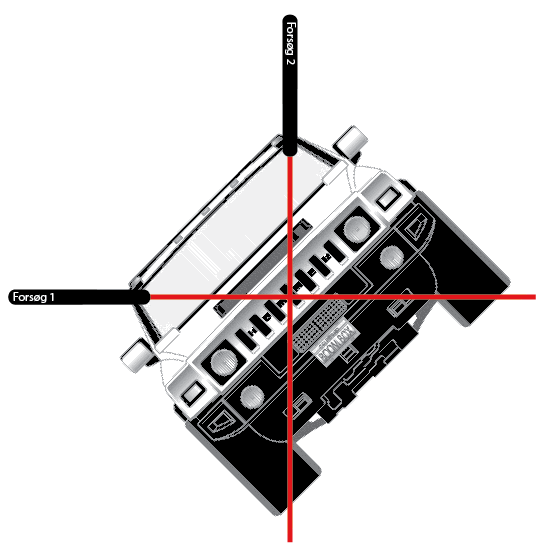
\includegraphics[scale=0.35]{./Graphics/massemidtpunkt.png}
\caption{Massemidtpunkt}
\label{massemidtpunkt}
\end{wrapfigure}

Efter at have fundet massemidtpunktet, måles afstanden fra punktet til banen. Denne distance benyttes herefter i en formel, der indikerer hvor hurtigt man kan køre i et sving.  \\

\( Fart(v) = (r*g*b/h)^\frac{1}{2} \), \\
r = radius,\\
g = tyngdekraft, \\
b = bilens bredde, \\
h = afstand mellem massemidtpunkt og banen. \\

For at optimere bilens fysiske egenskaber kan flere ting ændres. Opgaveformuleringen begrænser nogle muligheder såsom slibning af dæk, hvilket giver større overfladeareal og derved større friktion. \\

Derimod forbydes det ikke at justere bilens affjedring, hvilket giver ca. 3mm i massemidtpunktshøjde og derved højere teoretisk hastighed i svingene. Resultaterne for forskellige opsætninger kan ses i tabellen \ref{forskel_opsaat_result}. \\

\begin{table}[H]
\centering
\begin{tabular}{|l|l|l|}
\hline
Opsætning                      & Indre sving (m/s) & Ydre sving (m/s) \\ \hline
Standard u. perma,  u. elektro & 1,95              & 2,24             \\ \hline
Standard m. perma, u. elektro  & 2,64              & 3,03             \\ \hline
Standard u. perma, m. elektro  & 2,37              & 2,72             \\ \hline
Standard m. perma, m. elektro  & 2,87              & 3,30             \\ \hline
Sænket u. perma, u. elektro    & 2,12              & 2,43             \\ \hline
Sænket m. perma, u. elektro    & 2,86              & 3,28             \\ \hline
Sænket, u. perma, m. elektro   & 2,57              & 2,95             \\ \hline
Sænket, m. perma, m. elektro   & 3,12              & 3,58             \\ \hline
\end{tabular}
\caption{Forskellige opsætningers resultater}
\label{forskel_opsaat_result}
\end{table} 

Bredde af bil = \( 0,062m \), Svingradius Ydre = \( 0,33m \) \\
Svingradius Indre = \( 0,25m \), Tyngdekraft = \( 9,82m/s^2 \) \\
Permanent magnetkraft v. \( 2mm = 1,326N/8,1 m/s^2 \), \\
Elektromagnet v. \( 2mm = 0,9366N/4,7 m/s^2. \) \\  
Massemidtpunkthøjde = \( 0,02m \), Affjedring = \( [0;0,003m]. \) \\

Når det teoretiske maksimum er fundet skal resultatet implementeres i programmet. Da bilen ikke har et differentiale vil den decelerere i svinget. Derfor er det nødvendigt i programmet at tjekke den reelle hastighed bilen kører og sammenligne med den teoretiske. Dette gøres ved hjælp af omdrejningssensoren. Hvis der går for lang tid mellem pulsene øges bilens hastighed en smule. Hvis der går for kort tid mellem pulsene sænkes bilens hastighed en smule. Denne subrutine eksekveres gennem svinget således at hastigheden hele tiden reguleres til at være tættest på det teoretisk mulige. \\

\section{Bremse}
\label{bremse}
En stor del af optimeringen består i at finde det korrekte bremsepunkt. Jo senere der bremses jo hurtigere bliver omgangstiderne. For at finde disse bremsepunkter benyttes formlen: \\
\begin{align*}
V_f = V_i +2*a*d
\end{align*}
$V_f$ = maksimal fart i sving, $V_i$ = nuværende fart, a = deceleration(\(22.06m/s^2\)) og d = bremselængden. \\

Formlen benytter den maksimale teoretiske svinghastighed, bilens hastighed, deceleration og bremselængden. Da disse værdier ofte er kommatal, benyttes en lookup-tabel, som indeholder bremselængden som funktion af periodetiden fra omdrejningssensoren. \\

Lookup-tabellen i bilag \ref{lookup} tager udgangspunkt i en bestemt periodetid. Periodetiden benyttes til at udregnes hastigheden i $m/s$ og sættes ind i ovenstående formel. Konstanten A, er fundet ud fra et eksperiment, hvor bilen filmes mens den bremser. Videoen analyseres vha. programmet LoggerPro, som kan måle hastigheden og accelerationen. Ud fra disse værdier kan bremselængden findes. Denne måles i pulser, hvor det vides at 1 puls er lig med 0.005m. Dette er udregnet ud fra bilens gearing og hjulenes omkreds. Se afsnit \ref{beregn_gear} for beregninger.\\

Efter bilen har mappet banen benyttes lookup-tabellen til at finde det optimale bremsepunkt. Det gøres ved at tjekke omdrejningssensoren og sammenligne dennes værdi med værdierne i lookup-tabellen, for at finde bremselængden. Når afstanden til svinget er lig med bremselængde begynder bilen at bremse. Dette gøres ved at køre motoren baglæns indtil periodetiden i omdrejningssensoren er lig med den maksimale teoretiske periodetid for svinget. \\

Ud fra dette kan den optimale bremsedistance opnås og derved en hurtigere omgangstid. Da der kan være en del usikkerhed omkring testresultater osv. benyttes den optimale bremsedistance ikke i første omgang, da det kan resulterer i at bilen ryger af banen. I stedet øges bremsedistance i første omgang således at bilen med sikkerhed får sat en omgangstid. Herefter vil bilen i de følgende omgange nedsættes bremsedistancen indtil det teoretiske maksimum nås. \\
